%MIT OpenCourseWare: https://ocw.mit.edu
%RES.18-011 Algebra I Student Notes, Fall 2021
%License: Creative Commons BY-NC-SA 
%For information about citing these materials or our Terms of Use, visit: https://ocw.mit.edu/terms.

\section{Dimension Formula}
\subsection{Review}

Last time, we discussed linear transformations between two vector spaces. By picking a basis cleverly, it is possible to write the matrix of the linear transformation in a very nice form. For example, given a linear transformation $M: F^n \rto F^m,$ by changing the bases for $F^n$ and $F^m$ with the invertible matrices $P$ and $Q,$ the matrix $A$ will have a very simple form. 
\[
\begin{tikzcd}
F^n \arrow[r, "M"] & F^m \\
F^n \arrow[u, "P"]\arrow[r, "A"] & F^m \arrow[u, "Q"]
\end{tikzcd}
\]

With appropriate bases, 
\[
A = Q^{-1} M P = \begin{pmatrix} I_k & 0 \\ 0 & 0 \end{pmatrix},
\]

where $A$ is an $m \by n$ matrix with the identity in the top left corner. The first $k$ columns correspond to the image and the last $n - k$ columns correspond to the kernel. As a corollary, it is possible to see the \textbf{dimension formula} \[\dim \im (A) + \dim \ker(A) = n.\]

\begin{corollary}
Given a matrix $M \in \text{Mat}_{m \by n} (F),$ we have \[\text{rank}(M) = \text{rank}(M^T).\]
\end{corollary}

Essentially, this corollary states that the dimension of the span of the columns is the same as the dimension of the span of the rows, which is surprising! The first is a subspace of $F^m,$ while the second is a subspace of $F^n,$ but they still have the same dimension.
\begin{proof}[Sketch of Proof.]
This theorem is clearly true for $A,$ since the row-rank and the column-rank are both just $k$. However, since $A$ and $M$ differ by isomorphisms $P$ and $Q$, the rank of $A$ is the same as the rank of $M.$ Similarly, the rank of $A^T$ is also equal to the rank of $M^T.$ Therefore, \[\text{rank}(M) = \text{rank}(M^T).\]
\end{proof}

We are not going to use this often in this course, but this is a fact emphasized in traditional linear algebra classes. 

\subsection{Linear Operators}

Today, we will specialize the discussion on arbitrary linear transformations to \textbf{linear operators}, which go from a vector space to itself.

\begin{definition}
A \textbf{linear operator} is a linear transformation \[T: V \rto V.\] 
\end{definition}

Let's see some examples.
\begin{example}\label{rotation by theta}
Let $V = \RR^2.$ Then, $T$ is the linear transformation that is rotation by angle $\theta$ counterclockwise. This goes from the vector space to itself.
\end{example}

\begin{example}\label{derivative}
Let $V = \{\text{polynomials of degree} \leq 2\}.$ Then the derivative $T(f(t)) = f'(t)$ is a linear operator.
\end{example}

The first natural question to ask about linear operators is working out the matrix of the linear transformation upon picking a basis. The only difference between this discussion and the discussion on linear transformations is that here, the transformation is from a vector space to itself, so once a basis has been picked, both sides have a fixed basis. For general linear transformations from a vector space to a different vector space, two different bases can be picked. 

\begin{qq}
What is the matrix of a linear operator on a vector space with a chosen basis?
\end{qq}

Consider a basis \[B: F^n \rto V.\] Then $T$ becomes a square matrix $A \in \matnn(F).$ 

For Example \ref{rotation by theta}, picking the basis standard basis gives a rotation matrix: \[\left\{\begin{pmatrix}1 \\ 0\end{pmatrix}, \begin{pmatrix}0 \\ 1\end{pmatrix}\right\} \rightsquigarrow A = \begin{pmatrix} \cos\theta & -\sin\theta \\ \sin\theta & \cos\theta\end{pmatrix}.\] This is determined by figuring out where the $i$th basis vector is mapped, which is the $i$th column.

For Example \ref{derivative}, it is also possible to write down a matrix: \[\{1, t, t^2\} \rightsquigarrow A = \begin{pmatrix}
0 & 1 & 0 \\
0 & 0 & 2 \\
0 & 0 & 0
\end{pmatrix}.\]

This should all be reminiscent of the previous section. 

\begin{proposition}
When working with linear operators $T: V \rto V$, for $V$ finite-dimensional\footnote{In this class, the implicit assumption will always be that we are working with finite-dimensional vector spaces}, then \[T \text{ is injective }\leftrightarrow T \text{ is surjective }\leftrightarrow \text{ is an isomorphism.}\]
\end{proposition}

In fact, this fact is true for maps from a finite set to itself. Finite-dimensional vector spaces can be infinite, but have the same property.

\begin{proof}
Using the dimension formula, 
\[\dim \ker T + \dim \im T = \dim V.\] If $T$ is injective, then $\dim\ker T = 0,$ which is true if and only if $\dim\im T = \dim V,$ which means that $T$ is surjective. 
\end{proof}

So finite-dimensional vector spaces behave a lot like finite sets. 

\subsection{Change of Basis}

Now, the next natural question to ask is about changing bases. 
\begin{qq}
What happens to a matrix for $T: V \rto V$ upon changing basis for $V$?
\end{qq}

Specifying a basis for $V$ determines a diagram  \[
\begin{tikzcd}
V \arrow[r, "T"] & V \\
F^n \arrow[u, "B"]\arrow[r, "A"] & F^m \arrow[u, "B"]
\end{tikzcd}.
\]

A new basis comes from an invertible matrix $P \in GL_n(F)$, where the new basis is $B' = B \cdot P,$ and determines an extended diagram 
\[\begin{tikzcd}
V \arrow[r, "T"] & V \\
F^n \arrow[u, "B"]\arrow[r, "A"] & F^n \arrow[u, "B"] \\
F^n \arrow[u, "P"] \arrow[uu, bend left=49, "B'"] \arrow[r, "A'"] & F^n \arrow[u, "P"] \arrow[uu, bend right=49, "B'"]
\end{tikzcd}.
\]

There is a new matrix $A'$ that represents the same linear transformation $T.$ The difference between this case and the general case is that the bases are the same on either side of the transformation, and there is no longer the freedom to choose different bases for the domain and the codomain. 

The new matrix, by following the arrows on the diagram, is \[A' = P^{-1}AP.\] The matrix $A'$ is related to $A$ by conjugation by $P.$ 

\begin{definition}
A matrix $A'$ is \textbf{similar} to $A$ if there exists some $P \in GL_n(F)$ such that \[A' = P^{-1}AP.\]
\end{definition}
Similar matrices arise from the same linear operator from a vector space to itself, but with different bases picked. Again, to emphasize, the difference between today's case, $T: V \rto V$, and the case in the last section, $T: V \rto W$, is that in the first case there is only one base change matrix $P,$ instead of $P$ and $Q,$ since the matrix must operate the same on the left and right sides.


As an result, given a vector space $V$ and an operator $T: V \rto V,$ it is possible to define the determinant of $T$ \emph{without} having to specify a basis. The vector space $V$ might be a vector space without a canonical basis, but it is still possible to define the determinant. Picking any basis of $V$ produces a square matrix $A$, and the determinant would then be $\det(T) = \det(A).$ In fact, from the base change formula, it is clear that the determinant does not depend on which basis is used! From a different basis, \[\det(A') = \det(P^{-1}AP) = \det(P)^{-1}\det(A)\det(P) = \det(A),\] since the determinant is multiplicative. As a result, it is possible to define the determinant of $T$ independently of the choice of basis\footnote{It doesn't depend on which basis was chosen, so any basis works}, and so $\det(T)$ has a meaning outside of a particular basis. For example, on $\RR^n,$ the determinant represents a "volume," which is independent of the particular choice of basis. Here, we are saying that even for fields like finite fields, where "volume" may not make sense, the determinant still has some intrinsic meaning.

\subsection{Eigenvectors, Eigenvalues, and Diagonalizable Matrices}
Our discussion leads to the following question, which is the same as last class, but for linear operators.
\begin{qq}
How nice can we make $A$ by changing basis of $V$?
\end{qq}

Last class, it was possible to make the matrix extremely nice, since we could pick a basis for the domain \emph{and} for the codomain. Now, let's see an example for when the domain is the same vector space as the codomain. 

\begin{example}\label{diagonal matrix}
Let $V = \RR^2.$ Consider \[A = \begin{pmatrix} 2 & 3 \\ 3 & 2 \end{pmatrix}.\] We see that \[A \begin{pmatrix} 1 \\ 1 \end{pmatrix} = \begin{pmatrix} 5 \\ 5 \end{pmatrix} =  5\begin{pmatrix} 1 \\ 1 \end{pmatrix}\] and \[A\begin{pmatrix} -1 \\ 1 \end{pmatrix} = \begin{pmatrix} 1 \\ -1 \end{pmatrix} = -1 \begin{pmatrix} -1 \\ 1 \end{pmatrix}.\]

The operator is scaling the vector $(1, 1)$ and flipping the vector $(-1, 1),$ and the transformation on any other vector will be a combination of these two moves, scaling and flipping. In particular, taking \[P = \begin{pmatrix} 1 & -1 \\ 1 & 1\end{pmatrix},\] which has the first vector as the first column and the second vector as the second column, gives \[A' = P^{-1}AP = \begin{pmatrix} 5 & 0 \\ 0 & -1 \end{pmatrix}.\]

\begin{center}
    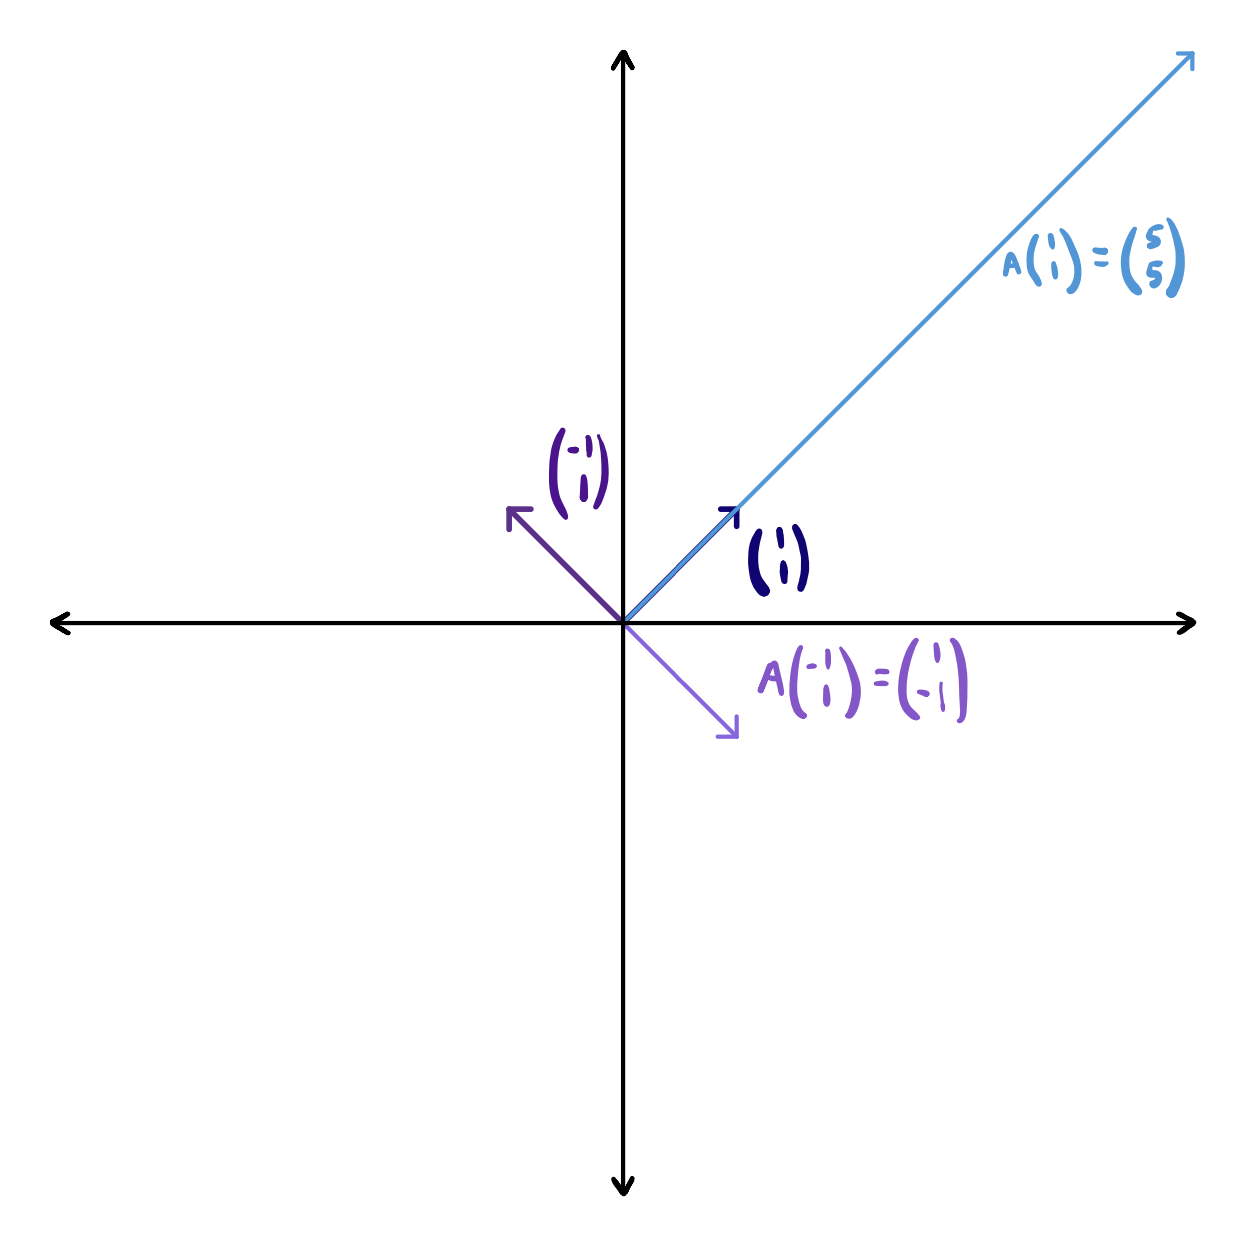
\includegraphics[width=8cm]{Lecture Files and Images/lec9-1.png}
\end{center}

\end{example}

In the new basis, it is possible to make the matrix diagonal! Making the matrix diagonal makes it possible to see how it operates, which is stretching by 5 in one direction, and flipping in the other direction (both independently of the other direction). 

In general, we will really want to be able to make matrices diagonal, since it allows us to see what it is doing in the direction of each basis vector, independently of the other directions (as there are 0s in the matrix elsewhere). This gold standard type of vector will be called an \textbf{eigenvector}.

\begin{definition}
A vector $v \neq 0$ is an \textbf{eigenvector} if \[Tv = \lambda v\] for some $\lambda \in F,$ and $\lambda$ is called an \textbf{eigenvalue}.
\end{definition}

When an operator is applied to a vector, the result is proportional to the vector. The operator maintains the direction of the vector, and just scales it. Obviously, scaling an eigenvector by some nonzero scalar also results in another eigenvector.

\begin{example}
For Example \ref{diagonal matrix}, the vector $\begin{pmatrix} 1 \\ 1 \end{pmatrix}$ is an eigenvector with eigenvalue 5, and $\begin{pmatrix} -1 \\ 1 \end{pmatrix}$ is an eigenvector with eigenvalue -$1.$
\end{example}

This example is special because not only are there eigenvectors, there are enough to form a basis. 

\begin{definition}
A basis $\{v_1, \cdots, v_n\}$ of $V$ where each $v_i$ is an eigenvector; that is, \[Tv_i = \lambda_i v_i,\] then the basis is called an \textbf{eigenbasis}.
\end{definition}

In an eigenbasis, the matrix for $T$ is \[\begin{pmatrix} \lambda_1 & \cdots & 0 \\
\vdots & \ddots & \vdots \\
0 & \cdots & \lambda_n\end{pmatrix},\] which is diagonal with $\lambda_i$ in the $(i, i)$th entry. 

Diagonal matrices are extremely nice. In general, it is very hard to take matrices to high powers, but for diagonal matrices, each entry is simply raised to that power.

\begin{definition}
If a linear operator has an eigenbasis $T,$ it is called \textbf{diagonalizable}.
\end{definition}

An equivalent definition holds for matrices.

\begin{definition}
Given a matrix $A,$ if there exists some invertible $P$ such that \[P^{-1}AP = D\] for some diagonal matrix $D$, then $A$ is called \textbf{diagonalizable}.
\end{definition}

That is, $A$ is diagonalizable if it is similar to a diagonal matrix. 

The key concept is that an eigenbasis provides the directions in which the operator $T$ behaves nicely by simply scaling or flipping a vector in that direction.
\subsection{Finding Eigenvalues and Eigenvectors}
 Unfortunately, not every matrix is diagonalizable, but the focus for the next few classes will be finding eigenvectors, eigenvalues, and eigenbases, assuming that a matrix \emph{is} diagonalizable.

\begin{qq}
How do we find eigenvectors, eigenvalues, and eigenbases?
\end{qq}

\begin{itemize}
    \item \textbf{Step 1.} Perhaps unintuitively, the first step is to find possible eigenvalues! Given a matrix $A \in \matnn(F)$ in some less good basis, we want to find eigenvectors that form a better basis that is an eigenbasis, so that $A$ will be diagonal and have a nicer form. 
    
    Suppose $\lambda$ is an eigenvalue for $A.$ Then there exists some nonzero $v$ such that \[Av = \lambda v,\] by definition. (There may be lots of $v,$ and in fact scaling any $v$ will produce another eigenvector, but for a given $\lambda$ we just want to know if there is a $v$ at all.) We know that \[\lambda v = \lambda I_n v,\] so this is equivalent to \[(\lambda I_n - A) v = 0\] for some $v.$ That is, the kernel is nontrivial: \[\ker(\lambda I_n -A) \neq \{\vec{0}\}.\] This is equivalent to \[\lambda I_n - A \text{ is not invertible,}\] which happens if and only if \[\det(\lambda I_n - A) = 0.\] This is not bad at all! The determinant is a formula that we can just calculate. 
    
    So in fact, we want to look for $\lambda$ such that the equation\[\boxed{\det(\lambda I_n - A) = 0}.\]  holds. It is customary in this context to replace $t$ with $\lambda,$ and so with $t$ as the variable, we have \[p(t) \coloneqq \det(t I_n - A),\] which is a polynomial of degree $n$ in $t$ called the \textbf{characteristic polynomial}.
    
    \begin{example}
    Given \[A = \begin{pmatrix} 2 & 3 \\ 3 & 2\end{pmatrix},\] we have the characteristic polynomial \[p_A(t) = \det\begin{pmatrix} t - 2 & -3 \\ -3 & t - 2\end{pmatrix} = (t-2)(t-2) - (-3)(-3) = t^2 - 4t - 5.\]
    \end{example}
    
    In general, where $A = (a_{ij}),$ we have \[p_A(t) = \det\begin{pmatrix} t - a_{11} & \cdots & \star \\
    \vdots & \ddots & \vdots \\
    \star & \cdots & t - a_{nn}
    \end{pmatrix} = t^n + \cdots ,\] which is a degree $n$ polynomial in $t.$
    
    If $A'$ is similar to $A,$ then they have the same characteristic polynomial, since the determinant is basis-invariant. 
    
    \begin{proposition}
    Given $\lambda \in F,$ $\lambda$ is an eigenvalue for $A$ if and only if $p_A(\lambda) = 0$; that is, if and only if $\lambda$ is a root of $p_A(t).$
    \end{proposition}
    
    For example, for our earlier example, the eigenvalues would be $-1$ and $5$, since $t^2 - 4t - 5 = (t + 1)(t - 5).$
    
    As a caveat, if $F$ is an arbitrary field, there may not be any roots. For example, a rotation matrix over $\RR$ does not have any real eigenvalues. However, if $F = \CC,$ there will always be $n$ roots (not necessarily distinct), and so there will always be eigenvalues. 
    
    \item \textbf{Step 2.} For each eigenvalue, find the associated eigenvectors. For each $\lambda,$ we want to take a vector in $\ker(\lambda I_n - A),$ which by assumption is a nonzero subspace. Using Gaussian elimination or row operations, we can mechanically compute a basis for $\ker(\lambda I_n - A),$ although we will not spend a lot of time on this. 
    
    \begin{example}
    For $\lambda = 5,$ we have \[5 \cdot I_2 - A = \begin{pmatrix} 3 & -3 \\ -3 & 3 \end{pmatrix},\] and the kernel is \[\ker = \spann \left\{\begin{pmatrix} 1 \\ 1 \end{pmatrix}\right\}.\]
    \end{example}
    
    We will say more about this next lecture!
\end{itemize}

\newpage